% 原文 pp.59–63（印刷 pp.1177–1181）

% 承接 p.58 末的 §4.3（Computation of the S-matrix）：此处继续构造满足 $\partial_+X_-=-\partial_-X_+$ 的算符对

% ===== 原文 p.59 =====
经典地，$X_+=T_{++}^2$ 满足上述条件，因为 $\partial_-(T_{++})^2=0$。然而在量子力学上，这个方程并不成立。于是我们将再次借助量纲计数（dimension counting）来论证守恒律的存在。

我们要证明：存在次数为 $(4,0)$ 与 $(3,1)$ 的算符 $X_+,X_-$，使得
\[
\partial_-X_++\partial_+X_-=0,\qquad X_+\ne\partial_+Y .
\]
为此，让我们把上面那张算符表扩充一下：
\[
\begin{array}{ll}
(3,0): & \partial_+\phi\,\partial_+^2\phi\\
(3,1): & (\partial_-\phi\,\partial_+\phi)(\partial_+\phi)^2,\quad \partial_-\phi\,\partial_+^3\phi,\\
(4,0): & \bigl((\partial_+\phi)^2\bigr)^2,\quad (\partial_+^2\phi)^2,\quad \partial_+^3\phi\,\partial_+\phi,\\
(4,1): & \partial_-\phi\,\partial_+^4\phi,\quad (\partial_-\phi\,\partial_+\phi)(\partial_+\phi\,\partial_+^2\phi),\quad (\partial_-\phi\,\partial_+^2\phi)(\partial_+\phi)^2.
\end{array}
\]

令 $H_{d_+,d_-}$ 为一切双次数（bidegree）为 $d_+-n,\ d_--n$（$n\ge0$）的算符所成的空间。我们有：$\dim H_{3,0}=1$、$\dim H_{3,1}=2$、$\dim H_{4,0}=3$、$\dim H_{4,1}=3$。我们有两个映射 $\partial_+:H_{3,1}\to H_{4,1}$ 与 $\partial_-:H_{4,0}\to H_{4,1}$。出于量纲上的理由，$H_{4,0}$ 中存在一个二维子空间 $Z$，使得对 $X\in Z$ 有 $\partial_-X\in\operatorname{Im}\partial_+$。另一方面，$\partial_+$ 在 $H_{4,0}$ 中的像 $B$ 是一维的。因此，那个「上同调」群 $H=Z/B$ 不为零（它是一维的）。这个「上同调」群所代表的，正是我们要找的守恒律。

% [Tutor Note: 此处「出于量纲上的理由」省略的其实是一段两行的线性代数，值得写清：$\partial_+$ 把一维的 $H_{3,0}$ 映入 $H_{4,0}$，故 $B=\operatorname{Im}\partial_+$ 是一维的；再看 $\partial_-:H_{4,0}\to H_{4,1}$ 复合上商映射 $H_{4,1}\to H_{4,1}/\operatorname{Im}\partial_+$（后者维数 $3-2=1$），得到一个线性泛函，其核即 $Z$，维数 $3-1=2$。第三步最容易被漏掉：必须验证 $B\subset Z$，而这恰好由 $\partial_-(\partial_+Y)=\partial_+\partial_-Y$（偏导数可交换）自动成立——用复形的语言说就是 $d^2=0$，故上边界必是闭上链。若 $\partial_+$ 与 $\partial_-$ 不对易（例如换成曲率非零的协变导数），$B\subset Z$ 便不再自动成立，$H=Z/B$ 连商空间都未必良定义，整个论证随之失效。]

\textbf{注（Remark）.} 很容易定义相应的复形，使 $Z$ 中元素为闭上链（cocycle）、$B$ 中元素为上边界（coboundary），而 $H$ 就是上同调。

把这个守恒律对应的荷算符记为 $Q$。设 $P_\pm$ 为 $x_+$、$x_-$ 平移的生成元，$K$ 为无穷小推促（boost）算符。由 $Q$ 的定义容易证明
\[
[Q,P_\pm]=0,\qquad [K,Q]=3Q .
\]
于是，$Q$ 是一个违背 Coleman–Mandula 定理结论的无穷小对称性。然而这个理论的 $S$ 矩阵并不等于 $1$；事实上 $S-1$ 是 $1/N$ 阶的量，并可用本讲第一部分所解释的 $1/N$ 展开算出。

% [Tutor Note: $[K,Q]=3Q$ 里的 $3$ 是本段最容易数错之处：$X_+$ 的双次数是 $(4,0)$，很自然会猜成 $[K,Q]=4Q$。但荷是对流形式 $J=X_+dx_+-X_-dx_-$ 积分而得：$Q=\int X_+dx_+$（沿 $x_-$ 为常数的类空切片积分）；由于 $\int dx_+dx_-$ 必须为双次数 $(0,0)$ 的不变量，$dx_+$ 自身带双次数 $(-1,0)$，故 $Q$ 的双次数是 $(3,0)$、自旋（即 $d_+-d_-$）为 $3$。换言之：$X_+$ 的 $4$ 个 $\partial_+$ 中有一个被 $dx_+$ 抵消掉。这个守恒荷因此是自旋 $3$ 的「高自旋」荷（与 Y. Y. Goldschmidt, E. Witten, Phys.\ Lett.\ 91B (1980) 392 所构造的高自旋守恒流一致）。]

\textbf{注（Remark）.} 当然，把 $Q$ 定义中的 $+$ 与 $-$ 互换，我们可以得到另一个「被禁戒的」守恒荷 $Q'$，满足 $[K,Q']=-3Q'$。

现在看看我们能怎样使用 $Q$。设 $H_m\subset H$ 是庞加莱群的一个子表示，它表示一个质量为 $m$ 的粒子（$H=L^2(\mathcal{O}_m^+)$）。设 $|k\rangle$ 记该粒子动量取 $k=(k_+,k_-)$ 的状态，其中 $k_+k_-=m^2$。（当然 $|k\rangle\notin H_m$；但对 $\mathcal{O}_m^+$ 上的 $L^2$ 函数 $f$，有 $\int f(k)|k\rangle dk\in H_m^+$。）我们有 $P_\pm|k\rangle=k_\pm|k\rangle$，以及
\[
Q|k\rangle=c\,k_+^3|k\rangle,
\]
其中 $c$ 是与 $k$ 无关的常数。$c$ 不为零这一点可在 $1/N$ 展开中显式算出。

% [Tutor Note: 这里的记号有两处原稿笔误（不影响论证）：(i) 括号中写 $H=L^2(\mathcal{O}_m^+)$，但按上下文定义的是单粒子子空间，应读作 $H_m=L^2(\mathcal{O}_m^+)$——同一句里 $H_m\subset H$ 已经把总希尔伯特空间记为 $H$，两者不能同名；(ii) 后一括号里的 $H_m^+$ 疑为 $H_m$ 之误（$\int f(k)|k\rangle dk$ 只是把 $H_m$ 的元素写成动量表象，并无额外的「$+$」空间）。此外 $\mathcal{O}_m^+$ 指前向质量壳双曲线 $\{k_+k_-=m^2,\ k_0>0\}$，而 $|k\rangle$ 是 $\delta$ 函数归一的「不可归一」态，故只能说它不属于 $H_m$，这正与 $\int f(k)|k\rangle dk$ 属于 $H_m$ 相对照。]

% [Tutor Note: $Q|k\rangle=c\,k_+^3|k\rangle$ 中的三次方并非任意：如上一批注所述 $Q$ 的双次数为 $(3,0)$，在洛伦兹群下只能按 $k_+^3$ 变换（等价地，$k\mapsto\Lambda k$ 时 $k_+\mapsto e^{\theta}k_+$，$Q$ 亦按 $e^{3\theta}$ 变换）。而「$c$ 与 $k$ 无关」的来源是 $[Q,P_\pm]=0$：$Q$ 与平移对易，故在每个给定质量 $m$ 的不可约表示上，$Q$ 只能是该表示上的一个固定标量；若让 $c=c(k)$ 依赖动量，就与 $[Q,P_\pm]=0$ 矛盾。反过来，$c$ 依赖粒子种类则是允许的——它由 $V$ 上的表示决定。]

设 $\lambda$ 为双曲线 $k_+k_-=m^2$ 上的参数，由方程 $k_\pm=me^{\pm\lambda}$ 定义。如我们所知，单粒子态由一个波函数表示，它满足 Klein–Gordon 方程：
\begin{equation}
  \tag{4.20}
  \label{eq:4-20}
  \psi(x_+,x_-)=\int_{-\infty}^{\infty}\widehat{\psi}(\lambda)e^{i(k_+x_++k_-x_-)}\,d\lambda,
\end{equation}

由于 $k_\pm=me^{\pm\lambda}$，(4.20) 中的指数是 $\lambda$ 的函数。假设我们考虑一个在位置与动量上都有适当局域性的波包，例如
\[
\widehat{\psi}(\lambda)=\exp\bigl(-(\lambda-\lambda_0)^2/\varepsilon\bigr)e^{if\lambda},
\]
其中 $\varepsilon$ 是小常数、$f$ 是常数，这就是一个合适的选择。(4.20) 中的波包近似地

% ===== 原文 p.60 =====
局域在一条经典轨道上，而该轨道可如下求出。积分的主要贡献来自 $\lambda$ 靠近 $\lambda_0$ 处，并且当 $x_\pm$ 使得被积函数的辐角在 $\lambda=\lambda_0$ 处驻定（stationary）时，积分取最大值。我把它留给读者去验证：这些条件确定的是一条直线，其速度依赖于 $\lambda_0$、位置依赖于 $f$。

% [Tutor Note: 作者说「留给读者验证」，省略的是标准的驻定相位计算：对 (4.20) 的指数 $\Phi(\lambda)=k_+x_++k_-x_-=m\bigl(e^{\lambda}x_++e^{-\lambda}x_-\bigr)$ 求驻定点，得 $\Phi'(\lambda)=m\bigl(e^{\lambda}x_+-e^{-\lambda}x_-\bigr)=0$，即 $x_+/x_-=e^{-2\lambda}$。在 $\lambda=\lambda_0$ 处它给出 $x_+/x_-=e^{-2\lambda_0}$：斜率（即速度）只由 $\lambda_0$ 决定。至于 $f$，它只出现在 $\widehat\psi$ 的相位 $e^{if\lambda}$ 中，相当于把 $\Phi$ 换成 $\Phi+f\lambda$，只改变驻定点方程中的常数项，故只平移轨迹位置、不改变斜率——这正是原文「$\lambda_0$ 决定速度、$f$ 决定位置」的来历。]

现在我们来计算「被禁戒的」对称性 $e^{i\delta Q}$ 如何作用在波函数上：
\begin{equation}
  \tag{4.21}
  \label{eq:4-21}
  e^{i\delta Q}\psi(x_+,x_-)=\int_{-\infty}^{\infty}\widehat{\psi}(\lambda)e^{i(\delta c\,k_+^3+k_+x_++k_-x_-)}\,d\lambda .
\end{equation}

我们仍可用驻定相位论证定出有效的经典轨道。这样做会发现：速度不受 $e^{i\delta Q}$ 影响，但 $x_+$ 的值被平移了
\[
\gamma_{\mathrm{eff}}=\delta c\,k_+^2,
\]
其中现在 $k_+=me^{\lambda_0}$。由于经典轨道的速度由 $\lambda_0$ 决定，位置的平移量就依赖于粒子的速度。这就是那个关键事实，它使确定 $S$ 矩阵成为可能；它也正是那些不具备 Coleman–Mandula 定理所述分解的玻色型对称性的特征性后果。

% [Tutor Note: 从 (4.21) 到 $\gamma_{\mathrm{eff}}=\delta c\,k_+^2$ 只做了一次重组，却极易差一个因子 $3$：注意 $k_+(\delta c\,k_+^2)=\delta c\,k_+^3$，故 (4.21) 指数中新增的 $\delta c\,k_+^3$ 可以并入 $k_+$ 的系数，读作 $k_+\bigl(x_++\delta c\,k_+^2\bigr)$，于是 $\delta c\,k_+^2$ 就是「有效的」$x_+$ 平移量。之所以它不是真正的平移，是因为 $k_+^2$ 随 $\lambda$ 变化：不同动量分量被平移了不同的量，这恰好使它能探测速度，而不只是把整个波包整体挪动。若因为 $\dfrac{d}{dk_+}(\delta c k_+^3)=3\delta c k_+^2$ 就把系数 $3$ 写进 $\gamma_{\mathrm{eff}}$，便错了——这里的 $k_+$ 是积分变量，不是可以自由求导的常数。]

$Q$ 这个对称性的存在还意味着：在两个入射粒子的散射中，末态必须恰好有两个粒子；并且若粒子标号正确，入射粒子的动量（从而质量）等于出射粒子的动量。的确，让我们暂时假定末态恰好有两个粒子。令 $1,2$ 标记入射粒子，$3,4$ 标记出射粒子。荷 $Q$ 作用在第 $i$ 个粒子的状态上，是乘上 $C_i(k_i)_+^3$。于是由荷守恒得
\[
C_1(k_1)_+^3+C_2(k_2)_+^3=C_3(k_3)_+^3+C_4(k_4)_+^3 .
\]
另一方面，由动量守恒得 $(k_1)_++(k_2)_+=(k_3)_++(k_4)_+$。因此，若 $k_1,k_2$ 已知，$(k_3,k_4)$ 就只能取一个离散的值集。再考虑到 $S$ 的解析性质，这就意味着 $(k_3,k_4)=(k_1,k_2)$ 或 $(k_3,k_4)=(k_2,k_1)$。同一类的论证还说明末态不可能多于两个粒子：$Q$ 守恒给出的关系，在初末态粒子数不同时，是一个解析的 $S$ 矩阵无法满足的。

% [Tutor Note: 上段把 p.59 的小写 $c$ 换成了带下标的 $C_i$，这一点值得停一下：对映入球面的 $\sigma$ 模型，$Q$ 由 $SO(N)$ 不变的算符构成，故 $[Q,SO(N)]=0$；于是 $Q$ 在不可约表示 $V$ 上必为标量（Schur 引理），$C_i\equiv c$ 与 $i$ 无关。原文保留 $C_i$ 的写法是为讨论更一般的（可能破坏 $SO(N)$ 的）情形。若误以为 $C_i$ 可以任意依赖于 $i$，下面由「荷守恒 + 动量守恒」推出 $(k_3,k_4)=(k_1,k_2)$ 或 $(k_2,k_1)$ 的论证就只剩一个离散条件、不再有唯一性；正是 $C_i\equiv c$ 使这两条守恒律联立后把结果锁死到这两个置换。]

% [Tutor Note: 「$(k_3,k_4)$ 只能取离散值集」到「$(k_3,k_4)=(k_1,k_2)$ 或 $(k_2,k_1)$」之间的跳步，作者在下段用 $S$ 的解析性补上了，其逻辑是：解析性禁止 $S$ 中出现除能量-动量守恒 $\delta$ 函数以外的任何 $\delta$ 函数，故守恒律给出的关系若真成立，就必须是动量守恒的代数推论而非额外的 $\delta$ 函数约束。做题时容易把这一步当成「由守恒律直接得到」，从而忽略解析性这个真正的前提。]

这些论证中对 $S$ 的解析性的用法，本质上如下。$S$ 的解析性不允许 $S$ 中出现除能量-动量守恒之外的任何 $\delta$ 函数。在两个入射、两个出射粒子的散射中，若（在正确标记粒子之后）初末质量相等，则能量-动量守恒就蕴含初末动量相等。于是，由 $Q$ 守恒得出的关系在这个情形下是一个恒等式（只要 $C_i$ 受到适当限制），而在其他情形下则不可能成立。

现在很容易解释 Coleman–Mandula 定理证明的想法，以及它在二维为何失效。

在一个具有「被禁戒的」对称性的理论中，若有两个粒子正走向碰撞（即它们的世界线相交；特别地，它们的速度不同），我们就可以施加这个「被禁戒的」对称性，把各粒子的位置平移依赖于速度、因而各不相同的量。在维数 $d>2$ 时，两条直线一般并不相交。在二维以上施加「被禁戒的」对称性，一般会得到两条不相交的世界线，而且可以让它们相距任意远。由于 $S$ 矩阵在该对称性下不变，能把 $S$ 矩阵的计算归结为世界线不相交的情形，就说明 $S$ 等于 $1$。

% ===== 原文 p.61 =====
\begin{figure}[htbp]
  \centering
  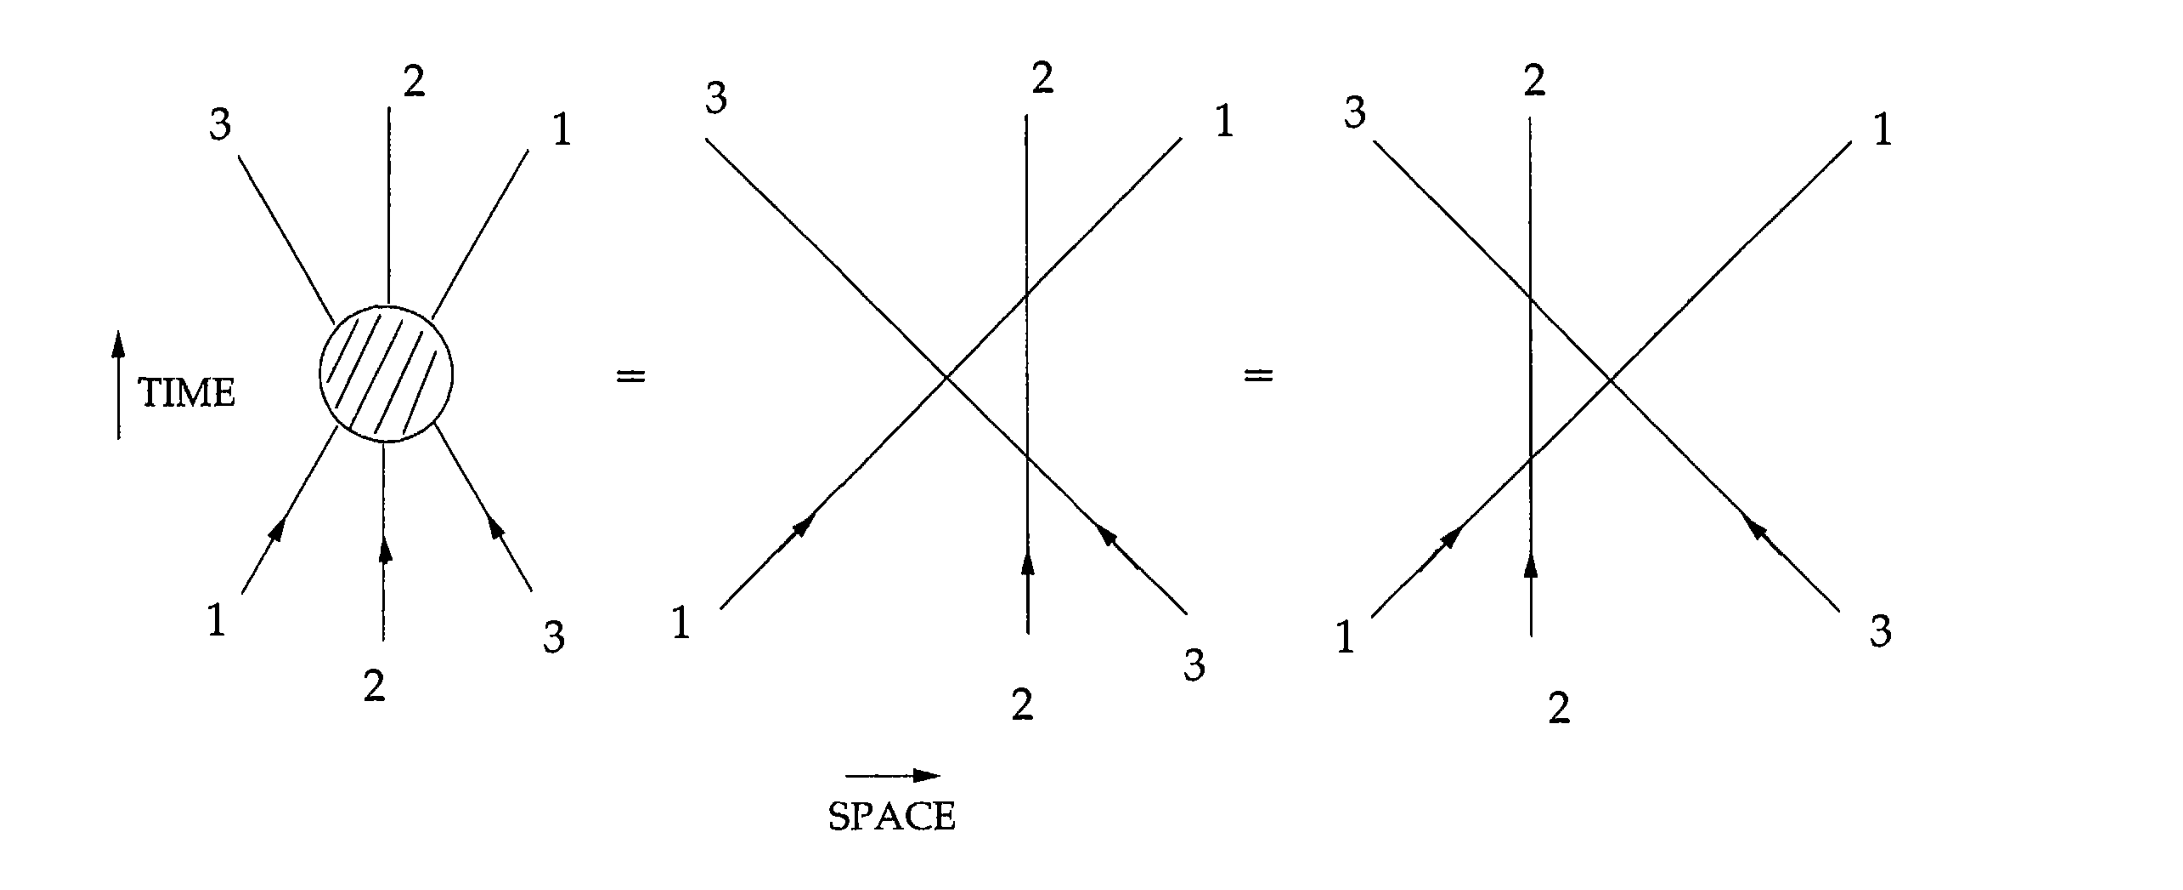
\includegraphics[width=0.78\textwidth]{figs/fig_p061_1.png}
  \caption{二维中三体散射约化为接连的三次两体碰撞。左：阴影圆盘表示一般的 $3\to3$ 散射；中、右：与它相等的两种图象，把该过程分解为三次 $2\to2$ 碰撞，两者的差别只在于这三次碰撞的先后次序（由「被禁戒」的对称性相联系）。纵轴为时间（TIME，向上），横轴为空间（SPACE，向右）；数字 $1,2,3$ 标记粒子，线上箭头指示动量方向。（原文 Figure 1，p.61；原图未给图号，此编号为本译本所加）}
  \label{fig:p061-1}
\end{figure}

然而在二维，两条直线一般是相交的，所以我们不能由上面的论证断定 $S$ 矩阵等于 $1$。不过，由于三条直线一般不会交于同一点，上面的论证表明：散射归结为（如图中所示）接连的三次两体碰撞，每一次都是两个粒子进、两个粒子出。这三次碰撞在时间次序上有两种可能，如图所示；而「被禁戒的」对称性意味着，对这两种时间次序，这三次碰撞相继发生的 $S$ 矩阵是相同的。

现在让我们回到靶空间为 $S^{N-1}$ 的 $\sigma$ 模型。在这个情形，如我们所知（对充分大的 $N$；并且我们相信对一切 $N>3$ 皆然），我们有 $N$ 个质量同为 $m$ 的有质量粒子，它们构成 $SO(N)$ 的一个 $N$ 维表示 $V$（即单粒子态空间是 $V\otimes L^2(\mathcal{O}_m^+)$）。上述论证允许我们对散射矩阵作出如下结论。

\subsection{映入 $S^{N-1}$ 的 $\sigma$ 模型的 $S$ 矩阵}

\noindent(i) $S$ 矩阵完全由「弹性两体散射（elastic two-body scattering）」决定，即由 $S$ 的两个入射、两个出射粒子的矩阵元决定。在这类散射中动量没有变化，所以 $S$ 矩阵约化成一个普通的矩阵值函数，即一个形如 $S(\lambda_1-\lambda_2)$、取值于 $\operatorname{End}_{SO(N)}(V\otimes V)$ 的函数，其中 $\lambda_i$ 由 $k_i=(me^{\lambda_i},me^{-\lambda_i})$ 定义，$k_i$ 是入射粒子的动量。（洛伦兹不变性意味着 $S$ 只依赖于差 $\lambda_1-\lambda_2$。）于是，$S$ 矩阵由如下形式的矩阵值函数显式描述：
\begin{equation}
  \tag{4.22}
  \label{eq:4-22}
  S(\theta)_{ij}^{kl}=F(\theta)\delta_i^k\delta_j^l+G(\theta)\delta_i^l\delta_j^k+H(\theta)\delta_{ij}\delta^{kl},
\end{equation}
其中 $F,G,H$ 是复值函数。

\noindent(ii) $S(\lambda)$ 满足量子 Yang–Baxter 方程：
\begin{equation}
  \tag{4.23}
  \label{eq:4-23}
  S_{12}(\lambda_1-\lambda_2)S_{13}(\lambda_1-\lambda_3)S_{23}(\lambda_2-\lambda_3)
  =S_{23}(\lambda_2-\lambda_3)S_{13}(\lambda_1-\lambda_3)S_{12}(\lambda_1-\lambda_2).
\end{equation}

\noindent(iii) 对任何实的 $\lambda$，$S(\lambda)$ 是幺正矩阵。

\noindent(iv) 交叉对称性（crossing symmetry）：$S$ 亚纯延拓到复平面，且
\[
S_{ij}^{kl}(\lambda)=S_{li}^{jk}(\pi i-\lambda).
\]

性质 (i) 我们基本上已经解释过；它就是「任何散射过程都由一串 $2\to2$ 过程决定，再加上 $SO(N)$ 对称性来约束 $2\to2$ 矩阵元」这一陈述。性质 (ii) 来自以下事实：$3\to3$ 散射矩阵分解为三个 $2\to2$ 散射
% ===== 原文 p.62 =====
矩阵之积，而这三次 $2\to2$ 碰撞发生的次序可以由图中的「被禁戒」对称性颠倒过来。性质 (iii) 对任何场论的 $S$ 矩阵都成立。性质 (iv) 称为交叉对称性，它是相对论场论的特征之一，在非相对论量子力学中没有对应物。粗略地说，它来自以下事实：$2\to2$ 的 $S$ 矩阵是四点函数极点的留数，而四点函数可以延拓到复的动量值。于是（由于庞加莱群的复化是连通的）$S$ 矩阵必须在庞加莱群的不连通分支下也不变，而该分支交换过去与未来，从而交换初态与末态粒子。（细节见去年秋季关于公理化的几讲。）

% [Tutor Note: 这里有一个容易读漏的指标结构，值得动手核一遍。把 (4.22) 看成 $V\otimes V$ 上的算子 $v^{ij}\mapsto S^{kl}_{ij}v^{ij}$，则它在三个不可约道上的本征值是：反对称道 $F-G$、对称无迹道 $F+G$、单态道 $F+G+NH$（后者的来历是 $\delta^{ij}\delta_{ij}=N$）。这个分解有两个用处：其一，可以立刻看出 (4.22) 的第三项必须写成 $\delta_{ij}\delta^{kl}$（两个下指标、两个上指标地配对），若写成 $\delta_i^j\delta^{kl}$ 之类则连指标类型都不对（多出一个上指标），$S$ 与 $SO(N)$ 对易这一条（即 (i) 中取值于 $\operatorname{End}_{SO(N)}(V\otimes V)$）也就无从谈起；其二，交叉对称性 $S^{kl}_{ij}(\lambda)=S^{jk}_{li}(\pi i-\lambda)$ 与 (4.22) 联立时，$F$ 项与 $F$ 项、$G$ 项与 $G$ 项、$H$ 项与 $H$ 项要各自配对，这正是 (4.24) 中三项之所以能共用一个标量因子 $f$ 的结构性原因。]

A. Zamolodchikov 与 Al. Zamolodchikov 于 1979 年证明：对 $N\ge3$，$S$ 矩阵被这些条件唯一确定，至多差一个依赖于 $\theta$ 的标量因子——前提是它非平凡（这一点我们可以从大 $N$ 展开得到）。在允许乘上一个对 $F,G,H$ 公共的标量函数 $f$ 的意义下，这个 $S$ 矩阵的 $F,G,H$ 由一个简单的显式公式给出：
\begin{equation}
  \tag{4.24}
  \label{eq:4-24}
  F(\theta)=1,\qquad G(\theta)=-\frac{2\pi i}{N-2}\,\theta,\qquad H(\theta)=-\frac{2\pi i}{(N-2)(\pi i-\theta)}.
\end{equation}

% [Tutor Note: 若把 (4.24) 当成完整的 $S$ 矩阵直接验证 (iii)（幺正性），会碰上一个真实的反例，值得记下来：取 $\theta=0$，则 $F=1$、$G=0$、$H(0)=-\frac{2\pi i}{(N-2)\pi i}=-\frac{2}{N-2}$；按上一条批注，(4.22) 的三个本征值是 $F-G=1$、$F+G=1$、$F+G+NH=1-\frac{2N}{N-2}$，最后一个对任何 $N>2$ 的模都不为 $1$（$N=3$ 时为 $-5$）。而 $f$ 对三项是公共因子，$\theta=0$ 时它只是一个数、只能把三个本征值同时缩放，故 $\{1,1\}$ 与 $1-\frac{2N}{N-2}$ 不可能被同时变成模 $1$——可见这不是「$f$ 尚未确定」造成的假象。因此 (4.24) 中分母 $N-2$ 值得核对：若换成 $N$，则 $H(0)=-2/N$，单态道本征值为 $1+NH(0)=1-2=-1$，于是 $\theta=0$ 处三个本征值 $\{1,1,-1\}$ 全在单位圆上，(iii) 立即成立。但 $N-2$ 在此处出现两次（$G$ 与 $H$），若真是排印之误应两处同改；稳妥的做法是把它记为原文存疑，对照 A. Zamolodchikov, Al. Zamolodchikov, Annals Phys.\ 120 (1979) 253 的原文核实后再定，不宜径改。另可注意 $H$ 在 $\theta=\pi i$ 处的极点正是交叉道的极点，这与 (iv) 中 $\pi i-\lambda$ 的平移互相印证，也说明 $(\pi i-\theta)$ 这个因子本身是对的。]

这个量子 Yang–Baxter 方程的解，是量子群（quantum group）理论据以发端的主要例子之一。与它相应的量子群现在称为「$\mathfrak{so}(N)$ 的 Yangian」（见 Drinfeld 在伯克利国际数学家大会上的报告「Quantum groups」）。

如我们已指出的，(4.24) 把 $S$ 矩阵确定到乘一个标量函数 $f(\theta)$ 为止。此外，这个函数满足条件
\[
f(\theta)f(-\theta)=1,\qquad f(\pi i-\theta)=f(\theta).
\]
因此 $f$ 是 $2\pi i$ 周期的。哪一个周期函数对应这个理论真正的 $S$ 矩阵，是一个不平凡的问题。微扰计算以及关于「简单性」的一般观念都强烈提示：这个函数应当这样选取，使得 $S$ 矩阵具有尽可能少的奇点。这样的选择有两个，其中之一被认为在 $\sigma$ 模型中实现；另一个选择被认为类似地在 Gross–Neveu 模型中实现。有趣的是，$f$ 不影响各反应的概率（因为对实的 $\lambda$ 它不影响 $F,G,H$ 的绝对值），但 $f$ 仍然重要，因为它影响散射过程中的「时间延迟」。

这样，我们就确定了映入 $S^{N-1}$ 的 $\sigma$ 模型的 $S$ 矩阵。人们也可以用这类论证确定该理论中算符在物理态之间的矩阵元（办法是写下 Yang–Baxter 方程的「表亲」方程，它们想必在量子群的语言中有其解释），但这一点我不打算讨论。

% [Tutor Note: 原文此处有一处排印重复：「One can show in a similar way the the Gross-Neveu model…」，多打了一个 the，应读作 the Gross–Neveu model。同一段还提到 Gross–Neveu 模型「用另一个极小的 $f$ 选择」得到其 $S$ 矩阵：这两个极小解分别对应 $\sigma$ 模型与 Gross–Neveu 模型，而它们在解析结构上的差别（极点分布不同）正是「$f$ 影响时间延迟却不影响概率」的具体体现——由于 $f$ 对 $F,G,H$ 是公共因子，各反应道之间的相对概率不变（这正是原文括号中那句话的稳妥读法），但散射的相移、从而时间延迟会改变。]

可以用类似方式证明：[I-Renorm Groups] 第 4 讲引入的 Gross–Neveu 模型同样是可积的，其意义与 $\sigma$ 模型相同。如我们已经提到的，它的 $S$ 矩阵是用另一个极小的 $f$ 选择得到的。

但映入球面的 $\sigma$ 模型与 Gross–Neveu 模型都是例外。在下一讲我们就会考虑一个稍复杂的 $\sigma$ 模型——靶空间为 $\mathbb{CP}^N$ 的模型，它不可积，其 $S$ 矩阵的显式形式未知，而且想必在某种意义上是无法知道的。

% ===== 原文 p.63 =====
在春季学期习题中有一个问题，要求证明以球面为靶空间的超对称 $\sigma$ 模型（supersymmetric sigma model）像它的玻色表亲一样可积。你还会在那个问题中看到：超对称 $\sigma$ 模型在某种意义上是普通 $\sigma$ 模型与 Gross–Neveu 模型的结合。顺便说一句，靶空间为 $\mathbb{CP}^N$ 的超对称模型也是可积的，尽管以该空间为靶空间的玻色 $\sigma$ 模型不可积。

\subsection{参考文献与交叉引用}

量子场论中散射的公理化在 [I-Axiomatics] 第 4 讲中讨论。二维 $\sigma$ 模型，特别是映入正曲率空间的二维 $\sigma$ 模型其 $\beta$ 函数为负这一事实，在 [II-CFT] 第 3 讲中讨论。Gross–Neveu 模型与本讲所讨论的非线性 $\sigma$ 模型密切相关，并有相似的 $1/N$ 展开，它在 [I-Renorm Groups] 第 4 讲中讨论。这些讲末尾的问题 3 与问题 4 涉及本文所述思想的超对称推广；问题 5 也涉及映入球面的 $\sigma$ 模型的大 $N$ 极限。

关于映入球面的 $\sigma$ 模型的高自旋守恒荷的构造，见
\begin{itemize}
  \item[] Y. Y. Goldschmidt, E. Witten, \textit{Conservation laws in some two-dimensional models}, Phys.\ Lett.\ \textbf{91B} (1980), 392.
\end{itemize}

关于 $\sigma$ 模型 $S$ 矩阵的计算，见
\begin{itemize}
  \item[] A. Zamolodchikov, Al. Zamolodchikov, \textit{Factorized $S$-matrices in two-dimensions as the exact solutions of certain relativistic quantum field models}, Annals Phys.\ \textbf{120} (1979), 253--291.
\end{itemize}

关于 Coleman–Mandula 定理在二维失效的直观讨论，以及若干精确 $S$ 矩阵的另外一些构造，见
\begin{itemize}
  \item[] R. Shankar, E. Witten, \textit{$S$ matrix of the supersymmetric nonlinear $\sigma$ model}, Phys.\ Rev.\ \textbf{D17} (1978), 2134.
\end{itemize}

% [Tutor Note: 文献条目按学术惯例保留原文（作者、篇名、卷号、页码），以便与原始文献对照；正文中的交叉引用代号 [I-Axiomatics]、[II-CFT]、[I-Renorm Groups] 分别指本丛书第 I 卷「公理化场论」、第 II 卷「共形场论」与第 I 卷「重整化群」的相应章节。注意 Goldschmidt–Witten 一文讨论的正是本讲 p.59 用数维度构造出的那个高自旋守恒荷（其自旋为 $3$），而 Shankar–Witten 一文给出的超对称非线性 $\sigma$ 模型 $S$ 矩阵是本讲 p.62 所说「两个极小 $f$ 选择」在超对称情形下的对应物。]
